%%%%%%%%%%%%%%%%%%%%%%%%%%%%%%%%%%%%%%%%%%%%%%%%%%%%%%%%%%%%%%%%%%%%%%%%
%                                                                      %
%     File: Thesis_Versat.tex                                      %
%     Tex Master: Thesis.tex                                           %
%                                                                      %
%     Author: Andre C. Marta                                           %
%     Last modified :  2 Jul 2015                                      %
%                                                                      %
%%%%%%%%%%%%%%%%%%%%%%%%%%%%%%%%%%%%%%%%%%%%%%%%%%%%%%%%%%%%%%%%%%%%%%%%

\chapter{The RV32-Versat Architecture}
\label{chapter:rv32-versat}

\newacro{CGRA}{Coarse-Grain Reconfigurable Array}

\begin{figure}[!htb]
	\centering
	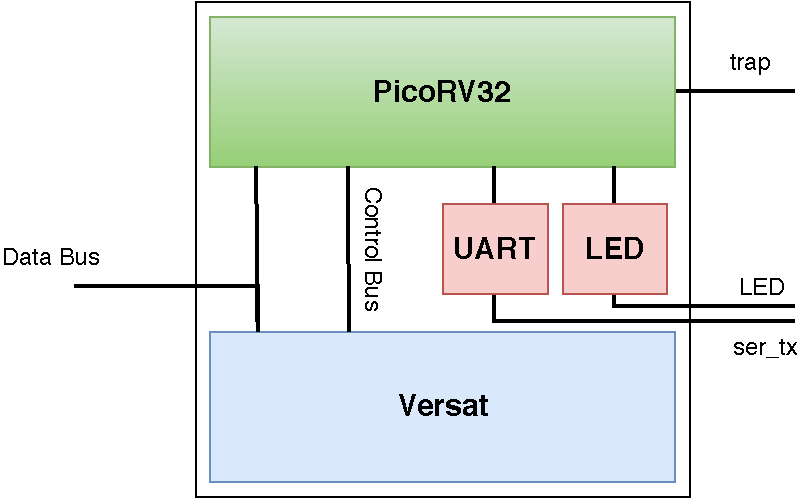
\includegraphics[width=0.8\textwidth]{Figures/rv32-versat.pdf}
	\caption{RV32-Versat top-level diagram.}
	\label{fig:rv32-versat}
\end{figure}

The RV32-Versat architecture was developed during this thesis, by a team of 3
people including the author. The starting point was the Versat
\ac{CGRA}~\cite{sousa:versat, sousa:versat2016, sousa:controller,
sousa:compiler, versat:specification}. A \acf{CGRA} is a collection of programmable 
\ac{FU} and embedded memories connected by programmable interconnects, forming the 
reconfigurable array. For a given set of configuration bits, the reconfigurable
array forms a hardware datapath that can execute an algorithm orders of magnitude faster 
than a conventional \ac{CPU}. This type of architectures can be used as hardware 
co-processors to accelerate algorithms that are time/power consuming in general purpose 
\ac{CPU}s.

The Versat \ac{CGRA} could only be programmed
in assembly language which, despite being great for optimising algorithms, it
was a problem when creating complex and lengthy algorithms. Thus, by removing
its controller (called PicoVersat) and replacing it by the PicoRV32
processor~\cite{cliffordwolf:picorv32}, with a RISC-V \ac{ISA}, this problem was
solved since now Versat can be programmed in the C/C++ language via the PicoRV32
processor. Versat will work as a peripheral of the processor for accelerating
parts of the program, using an interface of C++ classes created for this
purpose, as is explained in Section~\ref{subsection:c-driver}.

The RV32-Versat architecture is shown in Figure~\ref{fig:rv32-versat}, and it
comprises two main modules: the PicoRV32 processor and the Versat \ac{CGRA}.
There are also two additional modules in the RV32-Versat: the \ac{UART} and the
\ac{LED}.  Both modules are used for debugging. In this context the \ac{UART}
module is particularly useful, given that it allows to print values in the
computer terminal when simulating or testing the circuit. The LED provides an
even simpler debug mechanism when everything else fails.


As can be seen in the figure, the databus can be used to access the Versat's
memories with values from the PicoRV32 controller, external host or \ac{DMA}
master or, in simulation, by the testbench. This bus is used to upload
Versat with data to be processed and to download data already processed by
Versat. In case a testbench is used, hexadecimal files containing the input and
output data can be used, which is useful for debugging when developing new
applications. The data bus is comprised of the signals data databus\_sel (global
bus select), databus\_rnw (read / not write signal), databus\_addr (address),
databus\_data\_in (input data to PicoRV32) and databus\_data\_out (output data to
PicoRV32).

In RV32-Versat, Versat and the other cores are connected as memory mapped
peripherals of the PicoRV32 processor. This means that they are
accessed/programmed via the PicoRV32 bus, having dedicated memory addresses, as
shown in Table~\ref{tab:mem_map}, where the RV32-Versat memory map is shown.

\begin{table}[!htbp]
	\renewcommand{\arraystretch}{1.2} % more space between rows
	\caption{RV32-Versat memory map.}
	\label{tab:mem_map}
	\centering
	\begin{tabular}{ll}
		\toprule
		Peripheral     & Memory address\\
		\midrule
		\ac{UART} module    & 0x100\\
		\ac{LED} module     & 0x101\\
		Versat         & 0x110\\
		Versat databus & 0x120\\
		\bottomrule
	\end{tabular}
\end{table}

Other changes were made to Versat in order to adapt it for the RV32-Versat
architecture. One of these changes was the creation of a C++ driver, as detailed
in Section~\ref{subsection:c-driver}, that allows the user to program Versat
using C++ classes. For that, the user just needs to include the respective {\tt
  versatUI.hpp} header file and link the driver functions. This is a major
improvement, since previously Versat could only be programmed in Assembly,
whereas now it can be programmed using its C++ classes inside of a C or C++ code
that runs in the PicoRV32 processor. This is more user-friendly, as shown in the
application example of the Section~\ref{subsection:bprogramming}.

As detailed in Section~\ref{section:picorv32}, the PicoRV32 processor is far
from being a fast processor, since its main purpose is to be a small processor
with low power consumption. However, the impact that this has in the overall
performance of the system is attenuated by the use of Versat to speed up the
time consuming parts of the algorithms implemented in this system. This means
that the RV32-Versat is expected to have a performance similar to processors
with more resources (in terms of area and power consumption).


\section{The Versat architecture}
\label{section:versat}

\begin{figure}[!htb]
	\centering
	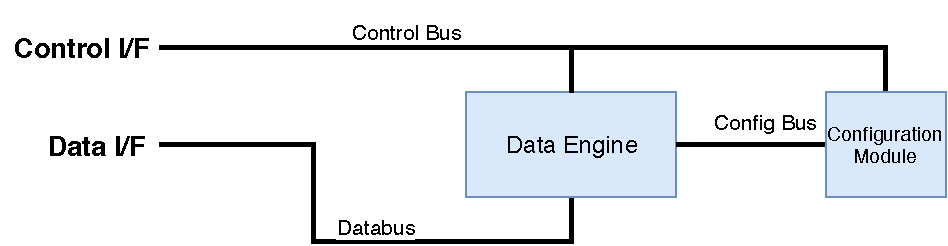
\includegraphics[width=0.8\textwidth]{Figures/top.pdf}
	\caption{Versat top-level entity.}
	\label{fig:top}
\end{figure}

The Versat CGRA architecture~\cite{sousa:versat, sousa:versat2016,
  sousa:controller, sousa:compiler, versat:specification} used in RV32-Versat is
shown in Figure~\ref{fig:top}, and it consists of two main modules: the Data
Engine and the Configuration Module. The Controller, Program Memory and Control
Register File that were previously included in the Versat architecture were
removed for the RV32-Versat system, given that in this new architecture the
Versat works as a peripheral, being controlled by the PicoRV32 processor.

The Versat core has a Control and a Data interface. The Control interface is
used by PicoRV32 processor to instruct Versat to load and execute programs. On
the other hand, the Data interface is used to load and read data from Versat.

Versat user programs can use the \ac{DE} to carry out data intensive computations. To
perform these computations, the PicoRV32 processor writes \ac{DE} configurations to
the \ac{CM}, through the host or memory interface, or simply restores
configurations previously stored in the \ac{CM}. The PicoRV32 can also load the
\ac{DE} with data to be processed or save the processed data back in the
external memory using the Data interface. This interface can also be used to
initially load the Versat program or to move \ac{CGRA} configurations between
the core and the external memory.


%%%%%%%%%%%%%%%%%%%%%%%%%%%%%%%%%%%%%%%%%%%%%%%%%%%%%%%%%%%%%%%%%%%%%%%%
\subsection{Data Engine}
\label{subsection:data}

\begin{figure}[!htb]
	\centering
	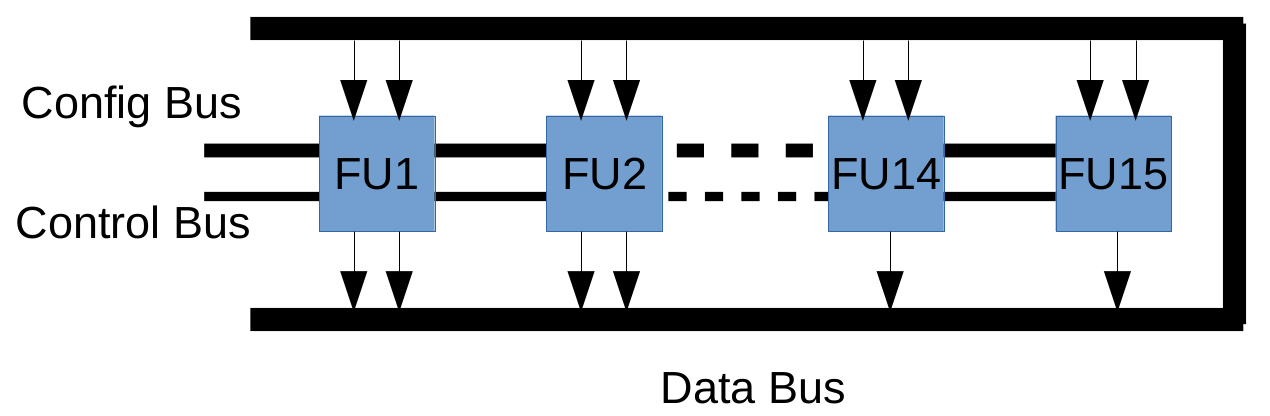
\includegraphics[width=0.8\textwidth]{Figures/de.png}
	\caption{Versat data engine.}
	\label{fig:de}
\end{figure}

The \ac{DE} has a flexible topology, in which the user can configure the number
of \ac{FU} and their respective types. In Figure~\ref{fig:de} it is shown a
\ac{DE} example with 15 \ac{FU}s. The \ac{DE} is a 32-bit architecture with the
following configurable \ac{FU}s: Arithmetic and Logic Unit (ALULite),
Multiplier Accumulator (Muladd), Barrel Shifter (BS) and dual-port 16kB embedded
memories (MEM).

The \ac{FU}s are interconnected by a wide bus called the Data Bus. This bus is
the concatenation of all \ac{FU} outputs, with each FU contributing with a
32-bit section to the Data Bus. An embedded memory contributes 2 sections to the
Data Bus, since it has 2 ports. The Data Bus allows for a maximum of 19
sections, and these sections can be selected by each FU, according to the
configurations that they receive from the respective configuration registers in
the \ac{CM}, whose outputs are concatenated in another wide bus called the
Config Bus.

The \ac{FU}'s have different latencies due to pipelining, as shown in
Table~\ref{tab:latencies} . As a result, when configuring a datapath those
latencies must be taken into account and compensated by configuring the Delay
parameter of the memories, as explained in Table~\ref{tab:agu}.

\begin{table}[!htb]
	\renewcommand{\arraystretch}{1.2} % more space between rows
	\caption{Latencies of the Versat FUs.}
	\label{tab:latencies}
	\centering
	\begin{tabular}{ll}
		\toprule
		Functional Unit & Latency\\
		\midrule
		Memory          &       1\\
		Barrel Shifter  &       1\\
		ALULite         &       2\\
		Muladd          &       3\\
		\bottomrule
	\end{tabular}
\end{table}

The \ac{DE} has a full mesh topology, meaning that each FU can select any
\ac{FU} output as one of its inputs. This kind of structure may seem unnecessary
but it greatly simplifies the compiler design as it avoids expensive place and
route algorithms~\cite{sousa:versat2016}. It also facilitates the configuration
of the different datapaths, because the user doesn't need to remember or check
what is connected to what since all the \ac{FU}s are interconnected.

%%%%%%%%%%%%%%%%%%%%%%%%%%%%%%%%%%%%%%%%%%%%%%%%%%%%%%%%%%%%%%%%%%%%%%%%
\subsubsection{ALULite}
\label{subsubsection:alulite}

The ALULite used in Versat has 2 data inputs (A and B), an output and 4
configuration bits. One of the configuration bits is used to create an internal
feedback loop from the output to the input A when activated (if the bit is set
to '0' there will be no feedback), meaning that an ALULite it can support up to
8 different operations. A list of this operations is shown in
Table~\ref{tab:alulite}.

\begin{table}[!htb]
	\renewcommand{\arraystretch}{1.2} % more space between rows
	\caption{ALULite operations.}
	\label{tab:alulite}
	\centering
	\begin{tabular}{lll}
		\toprule
		FNS & Operation              &              Operands\\
		\midrule
		000 & Addition               &             Y = A + B\\
		001 & Subtraction            &             Y = B - A\\
		010 & Signed compare         &       Y[31] = (A$>$B)\\
		011 & Multiplexer            &     Y = (A$<$0)? B: 0\\
		100 & Signed maximum         &            Y=max(A,B)\\
		101 & Signed minimum         &            Y=min(A,B)\\
		110 & Logic OR               &           Y = A $|$ B\\
		111 & Logic AND              &            Y = A \& B\\
		\bottomrule
	\end{tabular}
\end{table}

When the feedback loop is activated the input A of the ALULite can be used to
implement conditional statements in Addition, Subtraction, Multiplexer, Signed
maximum and Signed minimum operations. While the input A is not negative the
ALULite keeps accumulating the values coming to input B, stopping when the input
A has a negative value.

\subsubsection{Muladd}
\label{subsubsection:muladd}

The Multiply-Accumulate (Muladd) unit used in Versat has 3 data inputs (A, B and
O), an output and 3 configuration bits. The input O is used to control the
accumulation operations: if this input is different than 0, then the Muladd
keeps accumulating the multiplication results, otherwise the multiplier doesn't
accumulate the results. The Table~\ref{tab:muladd} shows the supported
operations.

\begin{table}[!htb]
	\renewcommand{\arraystretch}{1.2} % more space between rows
	\caption{Muladd operations.}
	\label{tab:muladd}
	\centering
	\begin{tabular}{lll}
		\toprule
		FNS & Operation   &                       Operands\\
		\midrule
		000 & MUL         &               Y = A $\times$ B\\
		001 & MUL\_DIV2   &      Y = (B $\times$ A)[63:32]\\
		010 & MACC\_16Q16 &  Y = Y + (B $\times$ A)[47:16]\\
		011 & MACC        &           Y = Y + B $\times$ A\\
		100 & MACC\_DIV2  &  Y = Y + (B $\times$ A)[63:32]\\
		101 & MSUB        &    Y = Y - (B $\times$ A)$<<$1\\
		110 & MSUB\_DIV2  &           Y =  Y - B $\times$ A\\
		111 & MUL\_LOW    &    Y = (Y + B $\times$ A)$<<$32\\
		\bottomrule
	\end{tabular}
\end{table}

\subsubsection{Barrel Shifter}
\label{subsubsection:bs}

The Barrel Shifter has 2 inputs (D for data and S for shift) and an output. This
functional unit can perform left and right shits, as shown in the
Table~\ref{tab:bs}, where the supported operations are listed. Two configuration
bits are used for this \ac{FU}, meaning that up to four operations are
available.

\begin{table}[!htb]
	\renewcommand{\arraystretch}{1.2} % more space between rows
	\caption{Barrel shifter operations.}
	\label{tab:bs}
	\centering
	\begin{tabular}{lll}
		\toprule
		FNS & Operation   &       Operands\\
		\midrule
		00  & SHR\_A      &   Y = D $>>$ S\\
		01  & SHR\_L      &  Y = D $>>>$ S\\%Rever notação!!!
		10  & SHL         &   Y = D $<<$ S\\
		\bottomrule
	\end{tabular}
\end{table}

\subsubsection{Memories}
\label{subsubsection:memories}

Each one of the dual-port memories used in Versat has a data input, a data
output and an address input, as shown in Figure~\ref{fig:memory}. The number of
memory positions is configurable, with each position having a fixed size of 32
bits.

Each one of the ports has an \ac{AGU} that can be programmed to generate the
address sequence used to access data from the memory port during the execution
of a program loop in the \ac{DE}. The \ac{AGU} support two levels of nested
loops and can start execution with a programmable delay, so that circuit paths
with different latencies can be synchronized.

\begin{figure}[!htb]
	\centering
	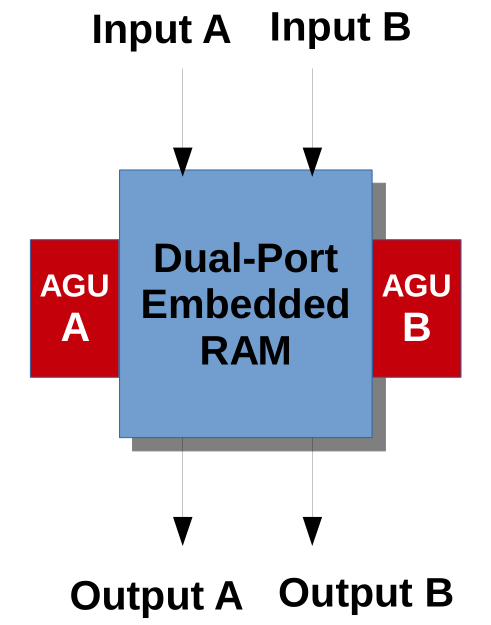
\includegraphics[width=0.23\textwidth]{Figures/memory.png}
	\caption{Versat dual-port embedded memory with AGU.}
	\label{fig:memory}
\end{figure}

Each \ac{AGU} has multiple configurable parameters, as detailed in
Table~\ref{tab:agu}, in order to control the address sequences generated. An
example address sequence is shown in Figure~\ref{fig:addrgen} , with the
\ac{AGU} configured with Start=10, Per=5, Duty=3, Incr=2, and Shift=-5, Delay=2,
and Reverse=0. Normally an \ac{AGU} is used for generating an address sequence
for the memory port. However, the port can be configured to output the generated
sequence to the DE, where it can be used.

\begin{table}[!htb]
	\renewcommand{\arraystretch}{1.2} % more space between rows
	\caption{AGU parameters.}
	\label{tab:agu}
	\centering
	\begin{tabular}{lcp{10cm}}
		\toprule
		Parameter & Size (bits) & Description\\
		\midrule
		Start     &          11 & Memory start address\\
		Per       &           5 & Number of iterations of the inner loop, aka Period\\
		Duty      &           5 & Number of cycles in a period (Per) that the memory is
		enabled\\
		Incr      &          11 & Increment for the inner loop\\
		Iter      &          11 & Number of iterations of the outer loop\\
		Shift     &          11 & Additional increment in the end of each period. Note 
		that
		Per+Shift is the increment of the outer loop\\
		Delay     &           5 & Number of clock cycles that the AGU must wait before 
		starting
		to work. Used to compensate different latencies in the converging branches of the
		configured hardware datapaths\\
		Reverse   &           1 & Bit-wise reversion of the generated address\\
		\bottomrule
	\end{tabular}
\end{table}

\begin{figure}[!htb]
	\centering
	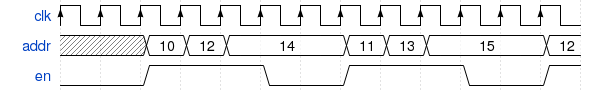
\includegraphics[width=0.75\textwidth]{Figures/addrgen.png}
	\caption{AGU output for Delay=2, Per=5, Duty=3, Start=10, Incr=2, Shift=-5 and 
	Reverse=0.}
	\label{fig:addrgen}
\end{figure}

The embedded memory ports also have their own configuration fields: one for
selecting/disabling the input generated sequence (Sel) and another for bypassing
the \ac{AGU} (Ext). When the memory input is disabled the respective port
becomes enabled for reading. Otherwise, when the input is selecting a data
source the port becomes enabled not only for writing but also for reading the
word previously stored at that address.

The configuration for bypassing the \ac{AGU} (Ext=1) enables the memory port
to use as address values computed by datapath. In this case the port address is
input by the other port of the same memory. This feature provides Versat with
the capability of working with pointers.

%%%%%%%%%%%%%%%%%%%%%%%%%%%%%%%%%%%%%%%%%%%%%%%%%%%%%%%%%%%%%%%%%%%%%%%%
\subsection{Configuration Module}
\label{subsection:configuration}

\begin{figure}[!htb]
	\centering
	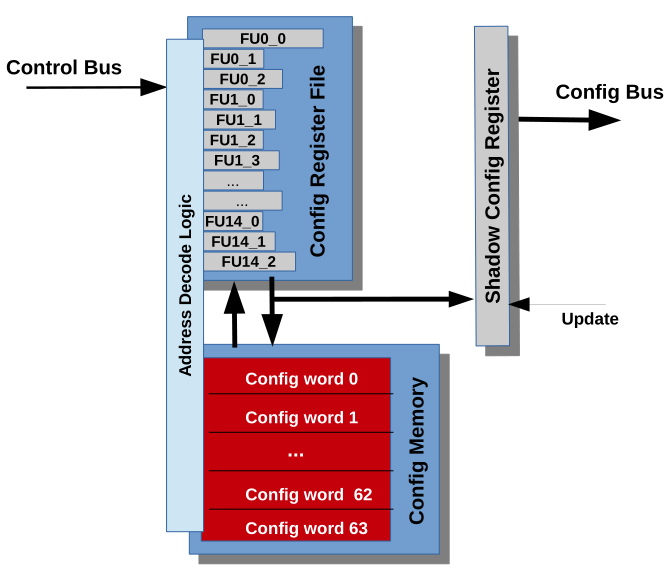
\includegraphics[width=0.6\textwidth]{Figures/configuration.png}
	\caption{Versat configuration module example.}
	\label{fig:cm}
\end{figure}

In Versat, the configuration bits are organized in configuration spaces, one for
each \ac{FU}. Each configuration space comprises multiple fields, which are
memory mapped from the Controller (PicoRV32) point of view. Thus, the Controller
is able to change a single configuration field of an FU by writing to the
respective address. This implements partial reconfiguration.

A \ac{CM} example is illustrated in Figure~\ref{fig:cm}, with a reduced number
of configuration spaces and fields for simplicity. It contains a register file
with a variable length (the length depends on the \ac{FU} used), a shadow
register and a memory. The shadow register holds the current configuration of
the \ac{DE}, which is copied from the main configuration register whenever the
Update signal is activated. This means that the configuration register can be
changed in the main register while the \ac{DE} is running.

When the \ac{CM} is addressed by the Controller, the decode logic checks if the
configuration register file or the configuration memory is being addressed. The
configuration register file accepts write requests and ignores read requests. On
the other hand, the configuration memory deals with read and write requests in
the following way: a read request causes the addressed contents of the
configuration memory to be transferred into the configuration register file,
while a write request causes the contents of the configuration register file to
be stored into the addressed position of the configuration memory. This is a
mechanism for saving and loading entire configurations in a single clock cycle
because all the data transfers are internal.

%%%%%%%%%%%%%%%%%%%%%%%%%%%%%%%%%%%%%%%%%%%%%%%%%%%%%%%%%%%%%%%%%%%%%%%%
\section{The PicoRV32 Architecture}
\label{section:picorv32}

The \ac{CPU} architecture used in the RV32-Versat system is the PicoRV32
architecture~\cite{cliffordwolf:picorv32}. It implements the RISC-V RV32IMC
instruction set and is publicly available under a free and open hardware
licence. This processor has a small size (750-2000 \ac{LUT} in 7-Series Xilinx
Architecture), and was originally meant to be used as an auxiliary processor in
\ac{FPGA} designs and \ac{ASIC}. Also, its high maximum frequency of operation
(250-450 MHz on 7-Series Xilinx FPGAs) means that it can be integrated in most
existing designs without crossing clock domains.

The \ac{CPI} numbers for the individual instructions can be found in
Table~\ref{tab:cpi}. It can be seen that the average CPI is approximately 4,
depending on the mix of instructions in the code, meaning that the PicoRV32 is
far from being a fast processor. However, this was already expected, since the
main purpose of this processor is to have a small area and power
consumption. Also, the high maximum clock frequency allowed by this processor
reduces the performance impact of the high \ac{CPI} figure.

\begin{table}[!htbp]
	\renewcommand{\arraystretch}{1.2} % more space between rows
	\caption{PicoRV32 CPI for different instructions.}
	\label{tab:cpi}
	\centering
	\begin{tabular}{ll}
		\toprule
		{\bf Instruction}   & {\bf \ac{CPI}} \\
		\midrule
		direct jump (jal)     &    3\\
		ALU reg + immediate   &    3\\
		ALU reg + reg         &    3\\
		branch (not taken) 	  &    3\\
		memory load           &    5\\
		memory store          &    5\\
		branch (taken)        &    5\\
		indirect jump (jalr)  &    6\\
		shift operations      & 4-14\\
		multiplication        &   40\\
		division              &   40\\
		multiplication (MULH) &   70\\
		\bottomrule
	\end{tabular}
\end{table}

%%%%%%%%%%%%%%%%%%%%%%%%%%%%%%%%%%%%%%%%%%%%%%%%%%%%%%%%%%%%%%%%%%%%%%%

\section{Programming RV32-Versat}
\label{section:programming}

As said before, the RV32-Versat can be programmed using C/C++, and the code can
be compiled using the GNU g++ compiler. To correctly configure Versat for
accelerating parts of the program, the C++ classes forming the Versat C++
driver, detailed in the next sub-section, must be included and used.

\subsection{C++ Driver}
\label{subsection:c-driver}

In order to allow the user to program Versat in an intuitive way using PicoRV32
as a controller, a driver was created. It consists of a C++ header file called
{\tt versatUI.hpp}, a C++ file file called {\tt versat\_func.cpp} and a python script 
called
{\tt xdictgen}. The {\tt versatUI.hpp} file, included in the {\tt versat\_func.cpp} file, 
contains multiple C++ classes, one for each type of functional unit, that contain
constructors that allow configuring the different functional units used in
Versat, as shown in Figure~\ref{fig:versatUI}. Each class was implemented with
multiple functions, this way allowing the configuration of only the necessary
parameters (instead of all the parameters), taking advantage of Versat's partial
reconfiguration capabilities.

When developing an application for the RV32-Versat, the user can configure the
Versat by using these classes directly in the C code that runs in the PicoRV32
processor. For example, in order to configure the ALULite parameters it can
simply write {\tt CALULite alulite0 (base, opa, opb, fns);}, where base,
opa, opb, fns are the configuration fields, and then write
{\tt alulite0.writeConf();} to write the configuration to alulite0. As
said before, partial reconfiguration is also supported, saving time in the
functional units reconfiguration. If the user wants, for example, to use the
same ALULite with the same inputs but performing a different operation, it just
needs to write {\tt alulite0.setFNS(fns)}, where fns is the desired
operation.

Besides the C++ classes, this file also includes the declaration of the function
{\tt defs}, used to initialize the constants that will hold the different
configuration addresses for each one of the configured Versat functional units.

In the file {\tt versat\_func.cpp} the functions used to configure and use the
Versat are declared. This way, the Versat can be easily configured directly from
the C code that runs in the PicoRV32 processor by calling this predefined
functions. The functions are the following:

\begin{itemize}
	\item \textbf{versatInit:} Function that checks if Versat is operational by writing
	something to its dummy register and reading it back. If the read value is equal to the
	written one, then Versat is working properly.
	\item \textbf{versatWriteConf:} Configures the Versat with the specified parameters. 
	For	example, if an ALULite is configured using 
	{\tt CALULite alulite0 (CONF\_ALULITE[0], sMEMA[0], sMEMB[3], ALULITE\_ADD);}, 
	this configuration can be written by calling {\tt ALULite0.writeConf();}.
	\item \textbf{versatClearConf:} Used to clear the current configurations of the 
	Versat by writing "0" to the {\tt CONF\_CLEAR} Versat address. This function must be 
	used 
	before configuring a new Versat kernel.
	\item \textbf{versatRun:} Function that runs the Versat \ac{DE}. First, it checks 
	if the \ac{DE} is ready by checking if the register that holds the data engine 
	status is "0". If it is, then it writes the value '1' to the register that runs the 
	data engine, otherwise it keeps waiting until the \ac{DE} is ready.
	\item \textbf{databusWrite:} Function used to write a value to a Versat memory 
	directly from the program
	\item \textbf{databusRead:} Loads a value from a Versat memory directly to the 
	program.
\end{itemize}

\begin{figure}[!htb]
	\begin{minipage}{\linewidth}
		\begin{spacing}{0.7}
			\begin{lstlisting}
			class CALULite {
				public:
				
				int base;
				int opa;
				int opb;
				int fns;
				
				CALULite (){
				}
				CALULite (int base, int opa, int opb, int fns) {
					this->base = base;
					this->opa = opa;
					this->opb = opb;
					this->fns = fns;
				}
				
				void writeConf() {
					RAM_SET32(VERSAT_TOP_BASE, (base  + ALULITE_CONF_SELA), opa);
					RAM_SET32(VERSAT_TOP_BASE, (base  + ALULITE_CONF_SELB), opb);
					RAM_SET32(VERSAT_TOP_BASE, (base  + ALULITE_CONF_FNS), fns);
				}
				void setOpA(int opa) {
					RAM_SET32(VERSAT_TOP_BASE, (this->base  + ALULITE_CONF_SELA), opa);
					this->opa = opa; 
				}
				void setOpB(int opb) {
					RAM_SET32(VERSAT_TOP_BASE, (this->base  + ALULITE_CONF_SELB), opb);
					this->opb = opb; 
				}
				void setFNS(int fns) {
					RAM_SET32(VERSAT_TOP_BASE, (this->base  + ALULITE_CONF_FNS), fns);
					this->fns = fns; 
				}
			};
			\end{lstlisting}
		\end{spacing}
	\end{minipage}
	\vspace*{-10mm}
	\caption{Example of a functional unit class declared in {\tt versatUI.hpp}.}
	\label{fig:versatUI}
\end{figure}

The {\tt xdictgen} python script was created to read the Versat Verilog include
files, extract the constants, and create a file called {\tt versat\_defs.hpp} with
all these constants. This file will then be included in the {\tt versatUI.hpp} file and
in the C code that runs in the PicoRV32 processor, making the Versat
configuration constants available in these files. This way, when configuring the
different functional units available, the user does not need to remember the
value of the different constants, instead she/he just needs to know their name.


\subsection{Basic Programming}
\label{subsection:bprogramming}

In order to better explain how the RV32-Versat is programmed, this section shows
an example program that writes values into two Versat memories, adds them and
then saves the results in another memory. The example program is shown in
Figure~\ref{fig:example}.

\begin{figure}[!htb]
	\begin{minipage}{\linewidth}
		\begin{spacing}{0.7}
			\begin{lstlisting}
			void main() {
				// setup uart
				uart_reset();
				
				//for 100MHz
				uart_setdiv(868);
				uart_wait();
				
				// init Versat
				uart_puts("Init Versat\n");
				defs();
				versatInit();
				versatClearConf(); //clean previous configurations
				
				//Write data to MEM0A and MEM1A
				databuswrite(ENG_MEM[0], 0, 1);
				databuswrite(ENG_MEM[0], 1, 2);
				databuswrite(ENG_MEM[0], 2, 3);
				databuswrite(ENG_MEM[1], 0, 4);
				databuswrite(ENG_MEM[1], 1, 5);
				databuswrite(ENG_MEM[1], 2, 6);
				
				//This kernel adds 3 numbers in Mem0 [0:2] with 3 numbers
				//of MEM1 [0:3] and saves the result in Mem2 [0:3]
				
				//Config MEM0 A to read data
				//mem0A (base, start, iter, incr, delay, per, duty, sel)
				CMem mem0A (CONF_MEMA[0], 0, 3, 1, 0, 1, 1, 0);
				mem0A.writeConf();
				
				//Config MEM1 A to read data
				CMem mem1A (CONF_MEMA[1], 0, 3, 1, 0, 1, 1, 0);
				mem1A.writeConf();
				
				//Config ALULITE
				CALULite alulite0 (CONF_ALULITE[0], sMEMA[0], sMEMA[1], ALULITE_ADD);
				alulite0.writeConf();
				
				//Config MEM2 A to save data
				CMem mem2A (CONF_MEMA[2], 0, 3, 1, 3, 1, 1, sALULITE0);
				mem2A.writeConf();
				
				//Run
				versatRun();
				
				uart_puts("Done\n");
			}
			\end{lstlisting}
		\end{spacing}
	\end{minipage}
	\vspace*{-10mm}
	\caption{Example program for RV32-Versat.}
	\label{fig:example}
\end{figure}

The program starts in the {\tt main} function, as usual in C or C++
programs, and the first thing it does is call the UART functions that in this
case will be used to print to the computer terminal. The function
{\tt uart\_reset} initializes the UART, the function
{\tt uart\_setdiv} sets the baud rate and the function
{\tt uart\_wait}, as the name indicates, waits until the \ac{UART} is ready.

After this the program proceeds to initialize the Versat, calling the functions
{\tt defs}, {\tt versatInit} and {\tt versatClearConf} that,
as explained previously in Section~\ref{subsection:c-driver}, initialize the
Versat and its data bus. When this is finished the memories of the Versat are
loaded with constants needed by the program (values 1, 2 and 3 for addresses 0,
1 and 2 of memory 0 and values 4, 5 and 6 for addresses 0, 1 and 2 of memory 1,
respectively). In this case, this was done directly in the C code, using the
function {\tt databusWrite}. However, for large sets of constants this is
not practical and the constants should instead be written into the memories via
the testbench of the RV32-Versat.

When the memory writing is finished the Versat's data engine is configured to
perform the desired operation, in this case adding the values previously stored
in the memories and saving them in memory 2. To do this, the classes defined in
the C++ driver (Section~\ref{subsection:c-driver}) are used. This way, the
memories are configured to perform 3 iterations, starting at address 0 and
incrementing by one address at the end of each iteration (see
Section~\ref{subsubsection:memories} for more details on the configuration
parameters of the memories).

The ALULite is configured to receive memory 0 and memory 1 as inputs, and to
have memory 2 as an output. The operation to be performed by the ALULite is also
configured, in this case it is the {\tt ALULITE\_ADD} operation. As explained in
Section~\ref{subsubsection:alulite}, this operation simply outputs the result of
the addition of the two inputs.

The last functional unit to be configured is memory 2 (note that this order was
chosen just to simplify the explanation, the configuration order does not
matter). Memory 2 is configured with the same parameters as memories 0 and 1: 3
iterations, starting at address 0 and incrementing by one address at the end of
each iteration.

After the configuration is finished function {\tt versatRun} is called in
order to run the data engine with the current configuration. When it finishes,
the {\tt uart\_puts} function is called to print in the pc terminal the
message "Done".


%%%%%%%%%%%%%%%%%%%%%%%%%%%%%%%%%%%%%%%%%%%%%%%%%%%%%%%%%%%%%%%%%%%%%%%%
\section{Application Example}
\label{section:application}

\begin{figure}[!htb]
	\centering
	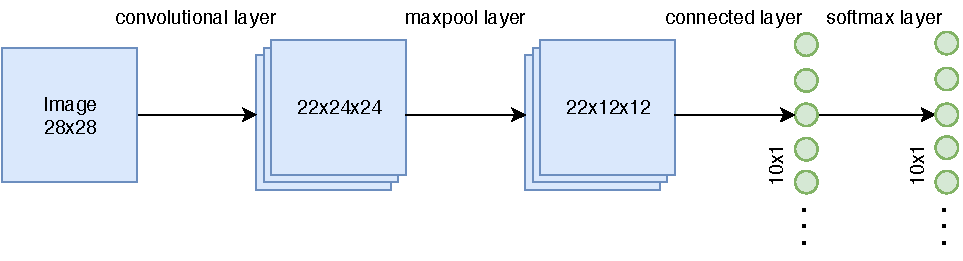
\includegraphics[width=0.9\textwidth]{Figures/CNN_architecture.pdf}
	\caption{CNN architecture implemented in RV32-Versat.}
	\label{fig:cnn}
\end{figure}

To fully test the system and the simulation environment an application using a previously
trained \ac{CNN} for digit classification in different images
was developed for the RV32-Versat. This application was based on a simple \ac{CNN} 
developed by the professor Horácio Neto for the Hardware/Software Co-Design course, and 
it consists of the following 4 layers, as shown in Figure~\ref{fig:cnn}:

\begin{itemize}
	\item \textbf{Forward convolutional layer:} This layer tests each feature map in each
	different position of the image. This is done through a convolution, by multiplying 
	each
	one of the feature's pixels by the respective image's pixel, and then adding these
	multiplications. At the end, this is divided by the total number of pixels of the 
	feature map.
	\item \textbf{Maxpool layer:} Here, each one of the matrices generated by the previous
	layer (24$\times$24) is scanned, and the maximum value of each 2$\times$2 region is 
	found. In the end, 22 matrices with dimension 12$\times$12 are obtained.
	\item \textbf{Fully connected layer:} The previously generated matrices go through a
	convolution process, being transformed into votes. These votes are expressed as 
	weights, determined by the network's previous training. In the end a 10 element 
	vector is generated	(one position for each number from 0-9), with each value 
	representing the amount of votes for that number.
	\item \textbf{Softmax layer:} This final layer use the previously obtained 10 elements
	and selects the position (and consequently the number) with the most votes. That 
	number is the final guess made by the network. Also, the vector is normalized and a 
	probabilistic distribution is made, being obtained the probability that the number 
	guessed is correct.
\end{itemize}

To adapt this application for RV32-Versat multiple changes were made. The first
change was to convert the program to fixed point (16Q16), since Versat only
works with fixed point numbers. Then, the forward convolutional and the fully
connected layers were rewritten using the Versat functions in order to
accelerate the execution of these layers.  The other layers were kept almost
unchanged, being executed in the PicoRV32 processor, since their execution time
was minimal when compared with the layers run in Versat.

After being implemented and fully tested, this application was used to benchmark
the different simulators after the simulation environment was developed. The
results are shown in Section~\ref{section:benchmark}.

From the four layers used in the implementation (forward convolutional, maxpool, fully
connected and softmax) only two were implemented using the Versat \ac{CGRA} (forward
convolutional and fully connected), with the two other layers being implemented in
software, since their execution time was minimal when compared with the other two layers.
As a result, the following functional units were used in Versat:
\begin{itemize}
	\item 4 dual-port memories with 65.5 KB each (262 KB in total)
	\item 2 Muladds
	\item 1 ALULite
\end{itemize}

In the following sections the datapaths created in Versat to accelerate the
execution of the forward convolutional and fully connected layers will be shown
and explained, along with the FU's configurations.

\subsection{Forward Convolutional Layer}
\label{subsection:fconvlayer}

This layer can be divided into three main parts: prepare the matrix A
({\tt prepare\_matrixA}), transpose the matrix B for and convolutionate it with A
({\tt fixed\_gemmBT}) and add the bias values and transpose the matrix
({\tt fixed\_add\_bias}).

In the {\tt prepare\_matrixA} function the matrix that contains the image
to be processed is transformed into a 25 $\times$ 24 $\times$ 24 matrix, making
it ready to be convolutioned with matrix B transposed. This transformation is
made by copying the values of the original matrix, contained in memory 0, to
multiple positions of the memory 3, as shown in Figure~\ref{fig:prepare_matrixA}.

\begin{figure}[!htb]
	\centering
	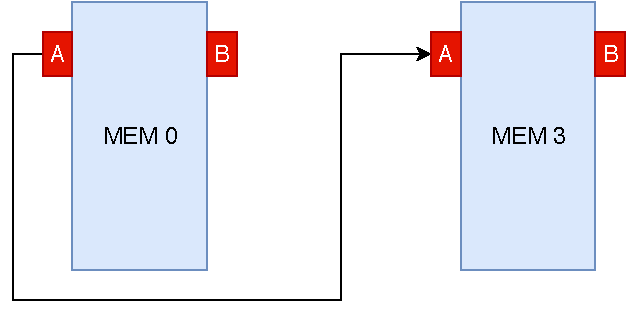
\includegraphics[width=0.5\textwidth]{Figures/prepare_matrixA.pdf}
	\caption{Datapath {\tt prepare\_matrixA}.}
	\label{fig:prepare_matrixA}
\end{figure}

The matrix A is then convolutioned with the transposed matrix B using the
Muladd, implementing the datapath shown in Figure~\ref{fig:fixed_gemmBT}. Both
the matrix A and the matrix B are stored in memory 3 (positions 0-14399 and
15022-15571, respectively), and sent to the Muladd. The memory 1 is used to
generate a counter between 0 and 25 that will be used to control the number of
accumulations done in the Muladd. This way, after accumulating 25
multiplications the Muladd accumulator will be reset, with memory 0 saving the
accumulation result in matrix C just before reset.

\begin{figure}[!htb]
	\centering
	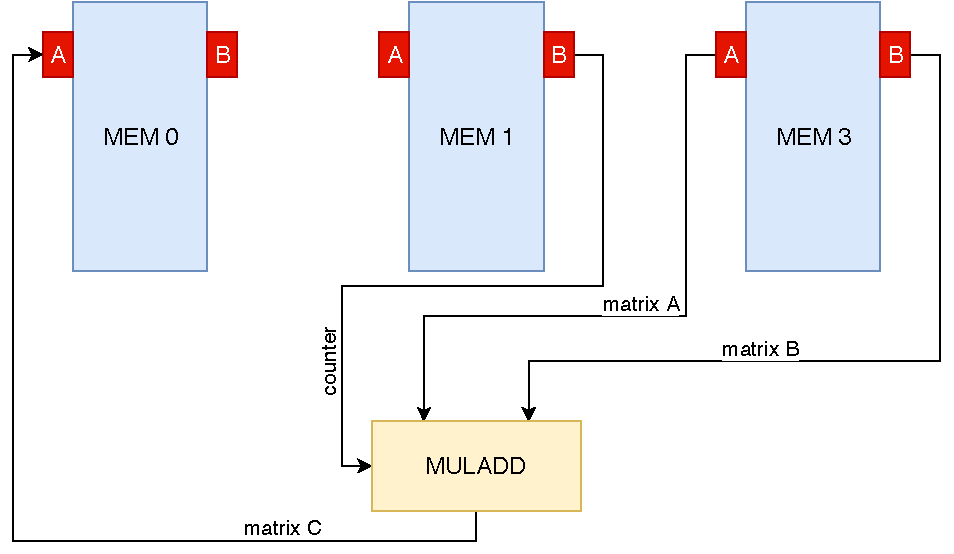
\includegraphics[width=0.8\textwidth]{Figures/fixed_gemmBT.pdf}
	\caption{Datapath {\tt fixed\_gemmBT}.}
	\label{fig:fixed_gemmBT}
\end{figure}

The matrix C previously obtained is transposed and sent to an ALULite, where the 22 bias
values, saved in memory 3 (positions 0-21) will be added. The resultant matrix (Cbias)
is saved in memory 3 through port A, as shown in Figure~\ref{fig:fixed_add_bias}

\begin{figure}[!htb]
	\centering
	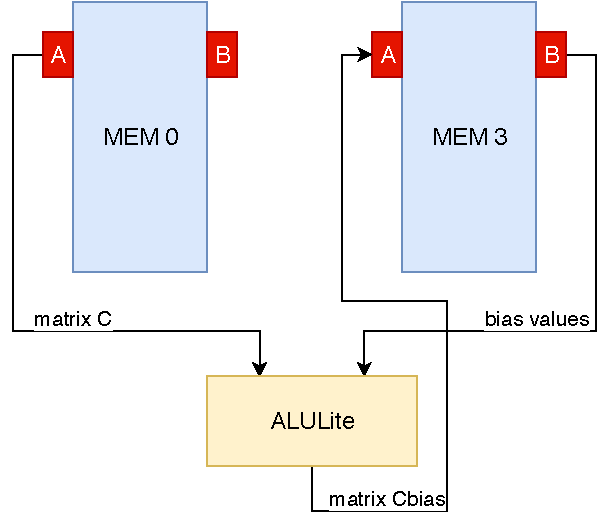
\includegraphics[width=0.5\textwidth]{Figures/fixed_add_bias.pdf}
	\caption{Datapath {\tt fixed\_add\_bias} in forward convolutional layer.}
	\label{fig:fixed_add_bias}
\end{figure}

\subsection{Fully Connected Layer}
\label{subsection:fconnlayer}

This layer can be divided into two main parts: the convolution of matrix Cpool
with matrix B ({\tt fixed\_gemm}) and the addition of the bias values to
the resultant matrix ({\tt fixed\_add\_bias}).

\begin{figure}[!htb]
	\centering
	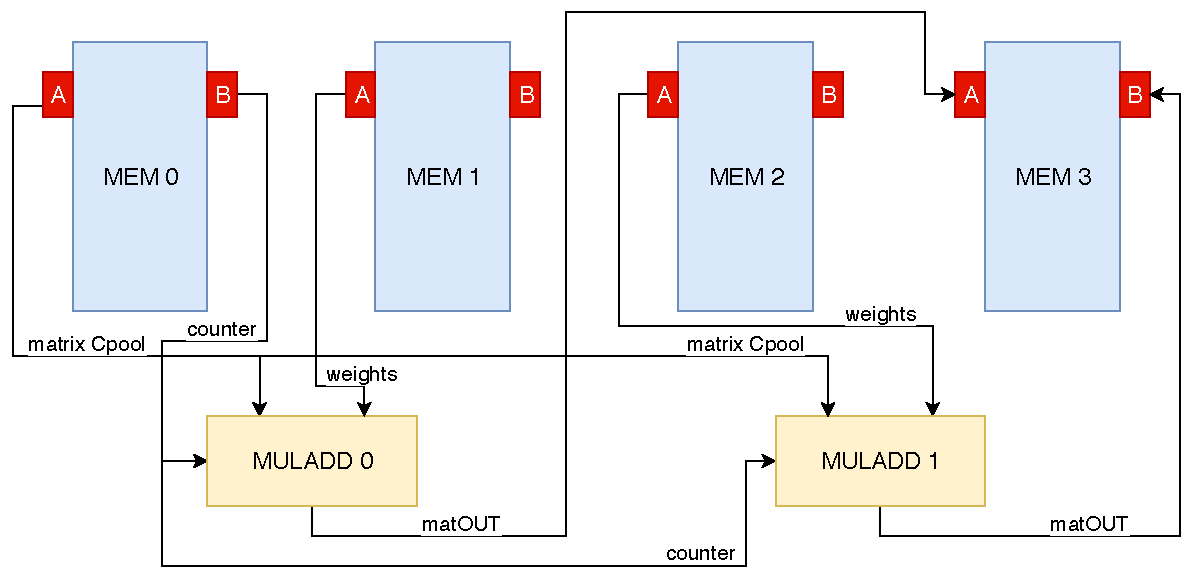
\includegraphics[width=1\textwidth]{Figures/fixed_gemm.pdf}
	\caption{Datapath {\tt fixed\_gemm}.}
	\label{fig:fixed_gemm}
\end{figure}

In {\tt fixed\_gemm} the convolution of matrix Cpool with the weights is
performed using two Muladds (Muladd 0 and Muladd 1), as shown in
Figure~\ref{fig:fixed_gemm}. Matrix Cpool is stored in memory 0, while the
weights are divided between memory 1 and memory 2 (the 32262 weights can not fit
inside a single memory). Memory 0 is used to generate a counter between 0
and 3168 that will be used to control the number of accumulations done in the
Muladds. This way, after accumulating 3168 multiplications the Muladd
accumulator will be reset, with memory 3 saving the accumulation result (matrix
matOUT) just before reset.

The use of two Muladds in this function allowed parallelization of the
algorithm, cutting its execution time by half (when compared with a non-parallel
run), and allowing it to be executed in a single run. If only a single Muladd
was used, two different datapaths would be needed: one to compute the first half
of matrix matOUT (using the weights stored in memory 1), and another to compute
the second half (using the weights stored in memory 2).

The {\tt fixed\_add\_bias} function is called again, but this time it will
add 10 bias values to matrix matOUT without transposing it, with the resultant
matrix ConnB being saved in the memory 0, as shown in
Figure~\ref{fig:fixed_add_bias_2}.

\begin{figure}[!htb]
	\centering
	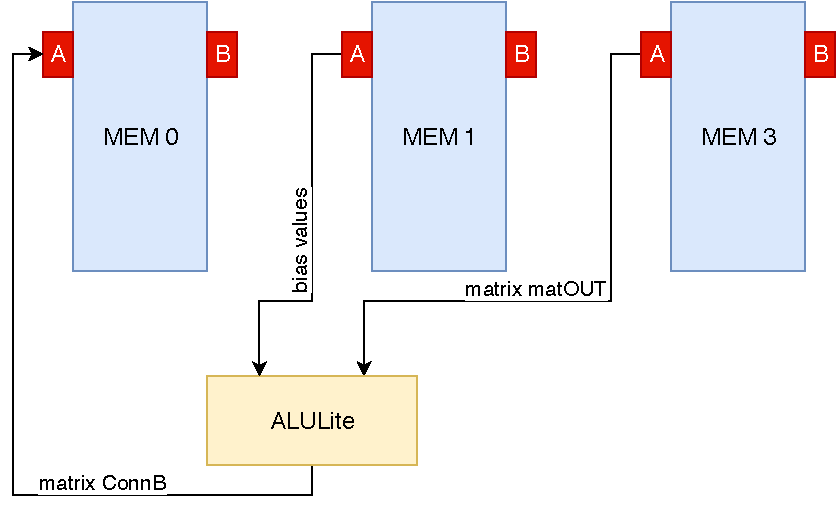
\includegraphics[width=0.7\textwidth]{Figures/fixed_add_bias_2.pdf}
	\caption{Datapath {\tt fixed\_add\_bias} in fully connected layer.}
	\label{fig:fixed_add_bias_2}
\end{figure}

